%%####################################################################
%    Copyright @ 2007 Andreas Frieß (Friess)
%    Permission is granted to copy, distribute and/or modify this document
%    under the terms of the GNU Free Documentation License, Version 1.2
%    or any later version published by the Free Software Foundation;
%    with no Invariant Sections, no Front-Cover Texts, and no Back-Cover Texts.
%    A copy of the license is included in the section entitled ``GNU
%    Free Documentation License''.
%%####################################################################
% Created: 21.08.2007
% @cvs($Date: 2007-09-05 19:46:18 +0000 (Wed, 05 Sep 2007) $)
% @cvs($Rev: 38 $)
% @cvs($Author: af0815 $)
% @cvs($URL: file:///svn/p/lazsnippets/code/trunk/dokumentation/LazSnippets/Kapitel/datenbanken/ProjektMySQLSimple.tex $)
%%####################################################################
\subsection{Projekt MySQLSimple}
\paragraph{Einleitung}
In diesem Projekt wird nur eine einfache Verbindung zur Datenbank aufgebaut und die grundlegenden Elemente die dafür notwendig sind erklärt. Es werden hierbei nur Elemente verwendet die bei einer Standardinstallation von Lazarus dabei sind.

\paragraph{Datenbank}
In der Datenbank muß für dieses Beispiel folgende Anweisung ausgeführt werden oder das ganze mittels des "`MySQL Query Browser" erstellt werden.
\begin{verbatim}
CREATE TABLE `laztest`.`ST_Person` (
  `STPerson` INTEGER UNSIGNED NOT NULL AUTO_INCREMENT \
     COMMENT 'Primaerschluessel',
  `cVName` VARCHAR(45) NOT NULL DEFAULT '' COMMENT 'Vorname',
  `cFName` VARCHAR(45) NOT NULL DEFAULT '' COMMENT 'Familienname',
  `cMName` VARCHAR(15) NOT NULL DEFAULT '' COMMENT 'Namensergaenzung',
  `cRName` VARCHAR(45) NOT NULL DEFAULT '' COMMENT 'Rufname',
  PRIMARY KEY (`STPerson`),
  UNIQUE INDEX `Namen_idx`(`cVName`, `cFName`, `cRName`)
)
ENGINE = InnoDB
CHARACTER SET latin1 COLLATE latin1_german1_ci
COMMENT = 'Personendaten';
\end{verbatim}
Wir erstellen hier einmal die für das Beispiel notwendige Tabelle für Personendaten. 
\parpic[sr][l]{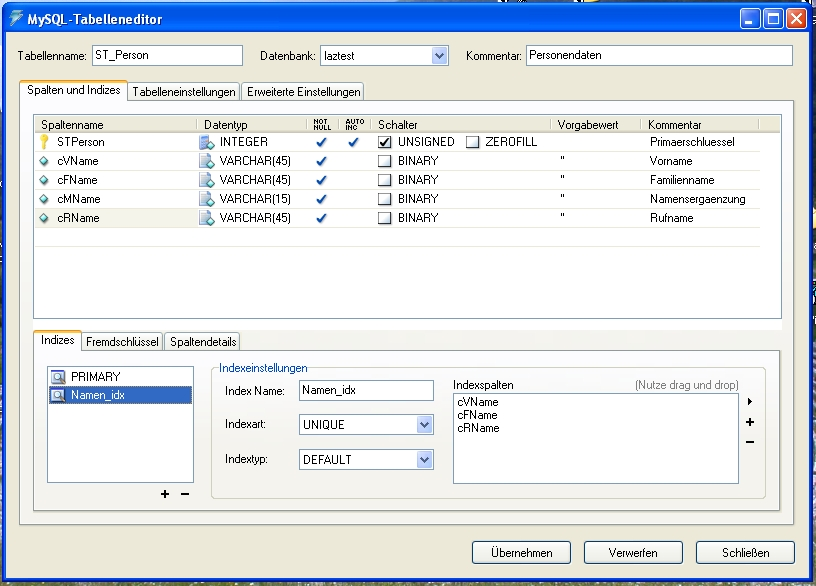
\includegraphics[width=0.35\textwidth]{Kapitel/datenbanken/pics/MySQLSimple02}}
\label{fig:MySQLSimple02}
Warum habe ich den Namen "`ST\_Person"' gewählt. Ganz einfach, ich rechne Tabellen mit diesem Inhalt zu den so genannten Stammdatentabellen. Das stimmt, außer wir haben hier eine reine Personenverwaltung. Nachdem das Beispiel aber erwitert werden soll, werden auch noch andere Tabellen folgen. 

Wir verwenden hier einmal die Spalte "`STPerson"' für den nicht Null  beinhaltenden (NOT NULL), automatisch hochzählenden (AUTO\_INCREMENT), eindeutigen Primärschlüssel (PRIMARY KEY ('STPerson')). In der Spalten "`cVName"' und "`cFName"' kommen der Vorname und der Familienname (=Nachname) hinein, zusätzlich gibt es noch das Feld für einen eventuelle Namensergänzung. Weiters beinhaltet die Spalte "`cRName"' noch den Rufnamen der Person.

Fast ganz unten in der definition der Tabelle befindet sich ein Hinweis auf einen weiteren Index. Dieser eindeutige Index (UNIQUE INDEX) soll verhindern, das gleiche Personen mehrmals in der Tabelle angelegt werden können. Warum wird dann aber nicht nur die Felder des Vornamens und des Familienanmens herangezogen ? Na, ja, was ist wenn wir mehrere "`Max Mustermann"' haben ! Im richtigen Leben hat man dann ja selbst noch hilfen, das zu unterscheiden. Dazu dient der Rufname (= Spitzname). Denn dann kannman den "`Max aus D"' und den "`Max aus A"' auch noch eintragen und die EInträge sind jetzt trotz der Namensgleichheit wirklich auseinander zu halten.

\paragraph{Benutzerschnittstelle}
Die Komponeneten kommen von der Palettenseite "`SQLdb"', "`DataAccess"' und "`DataControls"'.
\parpic[sr][l]{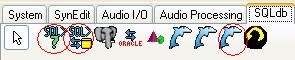
\includegraphics[width=0.35\textwidth]{Kapitel/datenbanken/pics/MySQLSimple01A}} \label{fig:MySQLSimple01A} 
Fangen wir einmal mit der "`SQLdb"' an. Um auf eine Datenbank zugreifen zu können, benötigen wir einmal eine Verbindungskomponente, das ist in unseren Fall eine der zur Datenbank passende Connection (= Verbindung). Da wir einen MySQL Server 5.x am laufen haben, so nehmen wir die passende "`MySQL50Connection"' Komponente und bringen sie auf das Projekt.
\parpic[sr][l]{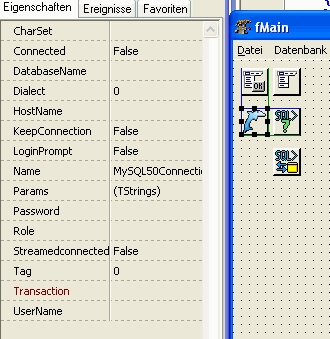
\includegraphics[width=0.25\textwidth]{Kapitel/datenbanken/pics/MySQLSimple03}} \label{fig:MySQLSimple03} 
Weiters fügen wir noch eine "`TSQLTransaction"' Komponente unserer Form hinzu.

Jetzt der Reihe nach, angefangen bei der "`TMySQL50\-Connection"' Komponente, müssen wir Einstellungen im Objektinspektor treffen. 

Bei der "`TMySQL50Connection"' Komponente sind es folgene Einstellungen. Der \textbf{DatabaseName} wird auf den Namen unserer Datenbank \emph{laztest} gesetzt. Der \textbf{HostName} ist bei einer kokalen installation immer \emph{localhost}. Für das \textbf{Paßwort} nehmen wir das des Benutzers, der sich mit der Datenbank verbindet. Bei \textbf{Transaction} müssen wir nur in das im Objektinspektor klicken und eine Auswahl erscheint. Wir nehmen hier unsere \emph{SQLTransaction1}. Als letztes geben wir den \textbf{UserNamen} ein, das ist ganz einfach der Benutzer den wir in der Datenbank erstellt haben, also \emph{lazarus@localhost}.

Die nächste Komponenete ist die "`TSQLTransaction"'. Dort müssen wir aktuell nichts einstellen, da sich die Eigenschaft \textbf{Database} im Objektinspektor bereits selbst auf \emph{MySQL50Connection1} geändert hat.

Den ersten Test kann man jetzt bereits durchführen. Durch anklicken der Eigenschaft \textbf{Connected} von \textbf{MySQL50Connection1} wechselt diese von \emph{False} auf \emph{True}. Wenn alles gut gelaufen ist, so läuft die Verbindung ohne Probleme ab. Wenn nicht, so muß man die Einstellungen nochmals überprüfen. Anschliessen stellen wir die Eigenschaft wieder auf \emph{False} zurück.

Nachdem die Verbindung zur Datenbank möglich ist, so müssen wir jetzt die Komponeneten für die Abfrage der Datenbank und die Anzeige der Daten noch hinzufügen. Es handelt sich hier um die Komponeneten "`TSQLQuery"' von Tab "`sqldb"', "`TDataSource"' vom Tab "`Data Access"' und "`TDBGrid"' vom Tab "`Data Controls"'.

Fangen wir mit der Komponente "`SQLQuery1"' an. Sie ist zuständig für die richtige Abfrage am Datenbankserver. Wir stellen die Eigenschaft \textbf{DataBase} auf unsere \emph{MySQL50Connection1} ein. Weiters müssen wir in die Eigenschaft \textbf{SQL} folgendes einfügen
\begin{verbatim}
SELECT `STPerson`, `cVName`, 
       `cFName`, `cMName`, `cRName`
  FROM st_person;
\end{verbatim}
und den Eigenschaftseditor wieder schließen. Die Eigenschaft hat sich \textbf{Transaction} im Objektinspektor bereits selbst auf \emph{SQLTransaction1} geändert. In der Komponenete "`Datasource1"' müssen wir nur \textbf{DataSet} per Mausklick auf \emph{SQLQuery1} einstellen. Als letztes konfigurieren wir das "`TDBGrid"'. Wir ändern mit der Maus die Eigenschaft \textbf{Align} auf \emph{alClient} und die Eigenschaft \textbf{DataSource} auf \emph{Datasource1}. Damit erfasst das Grid das komplette Formular. 

Prinzipiell ist unser Programm jetzt einmal optisch fertig. Wenn wir es jetzt kompilieren und laufen lassen, sehen wir das Formular, aber keine Daten und ändern können wir auch nichts. Es ist klar, wir haben die Komponenten konfiguriert, aber etwas Code wird auch benötigt um den Komponenten zu sagen, was wir wirklich wollen.

Dazu verwenden wir eine "`TActionList"' und ein "`TMainmenu"' aus dem Tab "`Standard"'. In der \textbf{ActionList1} erzeugen wir ganz einfach die Ereignisse \emph{actCloseDB}, \emph{actOpenDB} und \emph{actDataSetRefresh}. Ausserdem Erzeugen wir die Ereignisproceduren für das Form erzeugen un Form schliessen. Im MainMenu Komponente erzeugen dann ein kleines Menü.

\begin{verbatim}
procedure TfMain.actOpenDBExecute(Sender: TObject);
begin
  if not MySQL50Connection1.Connected then
  begin
    MySQL50Connection1.Connected := true;
  end;
  if not SQLQuery1.Active then SQLQuery1.Active := true;
end;
\end{verbatim}
Beim Eintreffen des Ereignisses für das Öffnen der Datenbank, wird als erstes Abgefragt ob die Verbindung bereits besteht. Ist die Verbindung vorhanden, so wird die Abfrage selbst geöffnet, falls sie noch nicht offen war.

\begin{verbatim}
procedure TfMain.actCloseDBExecute(Sender: TObject);
begin
  if MySQL50Connection1.Connected then
  begin
    if SQLQuery1.Active then
    begin
      SQLQuery1.ApplyUpdates;
      SQLQuery1.Active := false;
    end;
    MySQL50Connection1.Connected := false;
  end;
end;
\end{verbatim}
Wenn die Datenbank wieder geschlossen werden soll, so sind zuerst die noch nicht gespeicherten Daten zurückzuschreiben, dies geschieht mit dem Kommando \emph{ApplyUpdates}. Ohne diese Kommando bleiben die Änderungen nur lokal und werden mit der nächsten Abfrage wieder überschrieben. Anschliessend wird die Abfrage deaktiviert, dannach die Verbindung.

\begin{verbatim}
procedure TfMain.actDataSetRefreshExecute(Sender: TObject);
begin
  if not SQLQuery1.Active then exit;
  SQLQuery1.ApplyUpdates;
  SQLQuery1.Refresh;
end;
\end{verbatim}
Bei einer einfachen Auffrischung der Daten, arbeiten wir hier vorsichtshalber die Änderungen ein, bevor wir die eigentliche Auffrischung durchführen. Falls die Abfrage nicht aktiv war, brauchen wir klarerweise gar nichts zu machen.

\begin{verbatim}
procedure TfMain.FormDestroy(Sender: TObject);
begin
  actCloseDBExecute(Sender);
end;
\end{verbatim}
Wichtig ist, das beim Schließen des Formular, die Datenbankkomponenten wieder ordnungsgemäß von der Datenbank getrennt werden, ansonsten hat man Fehlermeldungen und auch blockierte Datenverbindungen. Generell sollte danch getrachtet werden, die Verbindungen, egal was geschieht, in konsistenten Zustand zu hinterlassen.

\paragraph{SVN}
Den Quelltext des Beispiel kann man sich auch mit folgenden Kommando aus dem SVN ind das aktuelle Verzeichnis holen.
\begin{verbatim}
svn co https://lazsnippets.svn.sourceforge.net/svnroot/lazsnippets/\
  trunk/datenbank/MySQL/MySQLSimple .
\end{verbatim}
Die Zeile ist in einem zu schreiben und wurde nur aus Formatierungsgründen hier beim Rückstrich (Backslash) umgebrochen. Der Punkt am Ende der Zeile ist notwendig, da es das Kennzeichen für das aktuelle Verzeichnis ist. Weiter ist auf die Schreibweise zu achten, das hier die Server zwischen Großbuchstaben und Kleinbuchstaben unterscheiden.
Die Datenbank muß man aber trotzdem selbst am MySQL Server erstellen. Die dazu benötigten Informationen befinden sich im Text von "`Datenbank"' weiter oben.

\paragraph{Version}
Derzeit ist das Beispiel mit der Version 0.9.23 beta von Lazarus entwickelt.
\begin{table}[htbp]
%	\centering
		\begin{tabular}[ht]{|l|l|}
      \hline
      Betriebssystem & getestet \\
      \hline
%      Linux Unbuntu & nein \\
      Linux Suse & nein \\
%      Linux Debian & nein \\
%      Win95 + WinME & nein \\
%      Win2k & nein \\
      WinXP & ja \\
%      WinVista & nein \\
      \hline
		\end{tabular}
\end{table}
\caption{Versionsübersicht}
\label{tab:MySQLSimpleVersion01} 

\verb|Version: $LastChangedRevision: 38 $ |\footnote{ Autor: Andreas Frieß\\Lizenz: GFDL}